% --------------------------------------------------------------
% This is all preamble stuff that you don't have to worry about.
% Head down to where it says "Start here"
% --------------------------------------------------------------
 
\documentclass[12pt]{article}
 
\usepackage[margin=1in]{geometry} 
\usepackage{amsmath,amsthm,amssymb,scrextend}
\usepackage{fancyhdr}
\usepackage{enumitem}
\usepackage{amsmath}
\usepackage{amssymb}
\usepackage{textcomp}
\usepackage{fancybox}
\usepackage{tikz}
\usepackage{tasks}
\pagestyle{fancy}
\usepackage[makeroom]{cancel}
\usepackage{graphicx}
\usepackage{caption}
\usepackage{mwe}
\usepackage{tikz}
\usetikzlibrary{positioning}

\newcommand{\N}{\mathbb{N}}
\newcommand{\Z}{\mathbb{Z}}
\newcommand{\I}{\mathbb{I}}
\newcommand{\R}{\mathbb{R}}
\newcommand{\Q}{\mathbb{Q}}
\renewcommand{\qed}{\hfill$\blacksquare$}
\let\newproof\proof
\renewenvironment{proof}{\begin{addmargin}[1em]{0em}\begin{newproof}}{\end{newproof}\end{addmargin}\qed}
% \newcommand{\expl}[1]{\text{\hfill[#1]}$}
 
\newenvironment{theorem}[2][Theorem]{\begin{trivlist}
\item[\hskip \labelsep {\bfseries #1}\hskip \labelsep {\bfseries #2.}]}{\end{trivlist}}
\newenvironment{lemma}[2][Lemma]{\begin{trivlist}
\item[\hskip \labelsep {\bfseries #1}\hskip \labelsep {\bfseries #2.}]}{\end{trivlist}}
\newenvironment{problem}[2][Problem]{\begin{trivlist}
\item[\hskip \labelsep {\bfseries #1}\hskip \labelsep {\bfseries #2.}]}{\end{trivlist}}
\newenvironment{exercise}[2][Exercise]{\begin{trivlist}
\item[\hskip \labelsep {\bfseries #1}\hskip \labelsep {\bfseries #2.}]}{\end{trivlist}}
\newenvironment{reflection}[2][Reflection]{\begin{trivlist}
\item[\hskip \labelsep {\bfseries #1}\hskip \labelsep {\bfseries #2.}]}{\end{trivlist}}
\newenvironment{proposition}[2][Proposition]{\begin{trivlist}
\item[\hskip \labelsep {\bfseries #1}\hskip \labelsep {\bfseries #2.}]}{\end{trivlist}}
\newenvironment{corollary}[2][Corollary]{\begin{trivlist}
\item[\hskip \labelsep {\bfseries #1}\hskip \labelsep {\bfseries #2.}]}{\end{trivlist}}
 
\setlength{\parindent}{0pt}
\begin{document}
 \settasks{
	counter-format=(tsk[r]),
	label-width=4ex
}
% --------------------------------------------------------------
%                         Start here
% --------------------------------------------------------------

\lhead{Math 475}
\chead{Homework 4}
\rhead{Meenmo Kang}

\begin{enumerate}
    \item[\bf 4.6.27] Generate the 3-subsets of \{1, 2, 3, 4, 5, 6\} in lexicographic order by using the algorithm described in Section 4.4.\\
    
    \begin{center}
        \begin{tabular}{cccc}
        (1,2,3) & (1,3,4) & (1,4,5) & (1,5,6) \\
        (1,2,4) & (1,3,5) & (1,4,6) &         \\
        (1,2,5) & (1,3,6) &         &         \\
        (1,2,6) &         &         &        
        \end{tabular}
    \end{center}
    
    \begin{center}
        \begin{tabular}{cccc}
        (2,3,4) & (2,4,5) & (2,5,6)&  \textcolor{white}{(0,0,0)}\\
        (2,3,5) & (2,4,6) &     &   \textcolor{white}{(0,0,0)}  \\
        (2,3,6) &         &      &  \textcolor{white}{(0,0,0)} 
        \end{tabular}
    \end{center}
    
    \begin{center}
        \begin{tabular}{cccc}
        (3,4,5)              & (3,5,6)              & \textcolor{white}{(0,0,0)} & \textcolor{white}{(0,0,0)} \\
        (3,4,6)              &                      & \textcolor{white}{(0,0,0)} & \textcolor{white}{(0,0,0)} \\
        \multicolumn{1}{l}{} & \multicolumn{1}{l}{} & \textcolor{white}{(0,0,0)} & \textcolor{white}{(0,0,0)}
        \end{tabular}
    \end{center}
    
    \begin{center}
        \begin{tabular}{cccc}
        (4,5,6) & \textcolor{white}{(0,0,0)} & \textcolor{white}{(0,0,0)} & \textcolor{white}{(0,0,0)} \\
        \textcolor{white}{(0,0,0)}     & \textcolor{white}{(0,0,0)} & \textcolor{white}{(0,0,0)} & \textcolor{white}{(0,0,0)} \\
        \textcolor{white}{(0,0,0)}     & \textcolor{white}{(0,0,0)} & \textcolor{white}{(0,0,0)} & \textcolor{white}{(0,0,0)}
        \end{tabular}
    \end{center}
    
    \item[\bf 5.7.1] Prove Pascal's formula by substituting the values of the binomial coefficients as given in equation (5.1).\\
    
    \begin{align*}
        %\binom{n-1}{k-1}+\binom{n-1}{k} &= \frac{(n-1)!}{(k-1)!(n-k)!}+\frac{(n-1)!}{k!(n-1-k)!}
        \binom{n}{r} &= \frac{n!}{(n-r)!r!} = \frac{n(n-1)!}{(n-r)!r!}\\
                     &= \frac{(n-1)!(n-(r-r))}{(n-r)!r!} = \frac{(n-1)!(n-r)}{(n-r)!r!} + \frac{(n-1)!r}{(n-r)!r!}\\
                     &= \frac{(n-1)!}{(n-r-1)!r!} + \frac{(n-1)!}{(n-r)!(r-1)!}\\
                     &= \binom{n-1}{r} + \binom{n-1}{r-1}
    \end{align*}

    
    \newpage
    \item[\bf 5.7.3] Consider the sum of the binomial coefficients along the diagonals of Pascal's triangle running upward from the left. The first few are 1,\; 1,\; 1 + 1 = 2,\;1 + 2 = 3,\; 1 + 3 + 1 = 5,\; 1 + 4 + 3 = 8. Compute several more of these diagonal sums, and determine how these sums are related.\\
   
$$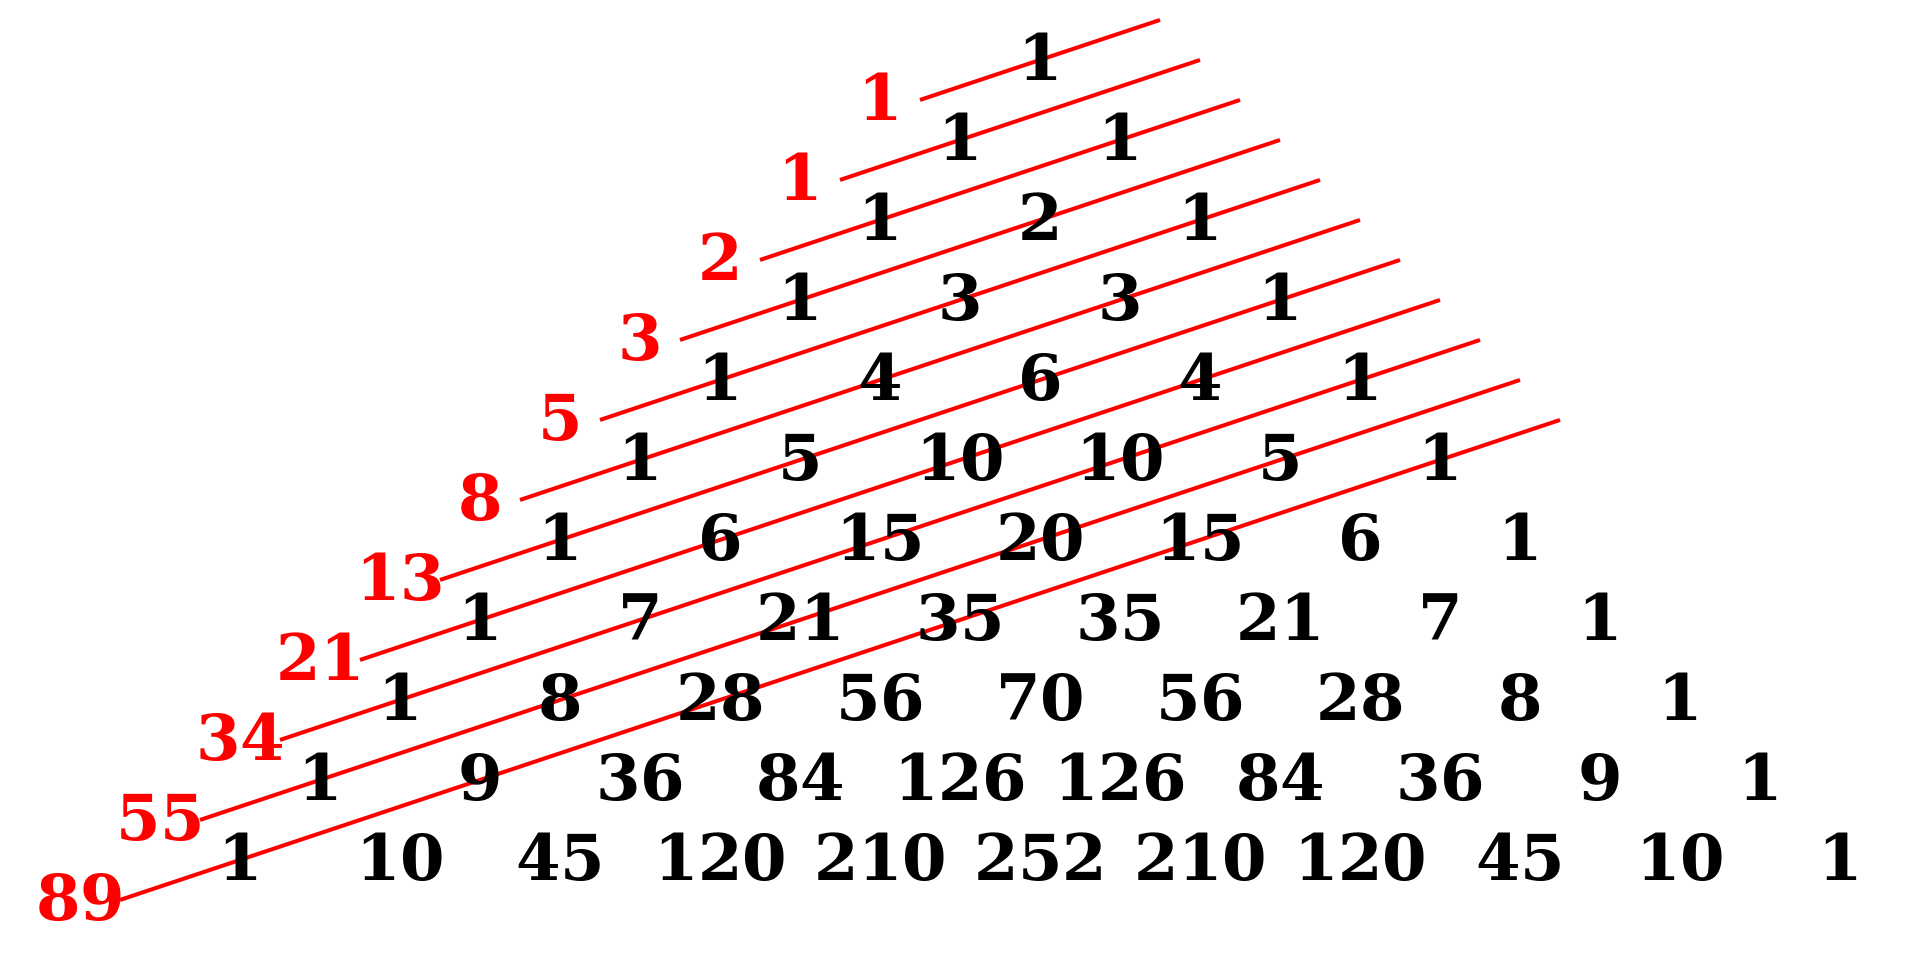
\includegraphics[height=4cm, width=7cm]{Homework/fibo.png}$$

    
    I found a rule on the sum of the binomial coefficients which is 
    \begin{align}
    a_n=a_{n-1}+a_{n=2} \tag{for $n\ge 2$}
    \end{align}
    
    \vspace{1.5\baselineskip}
    \item[\bf 5.7.4] Expand $(x+y)^5$ and $(x+y)^6$ using the binomial theorem.\\
    \begin{align*}
        (x+y)^5 &= \binom{5}{0}x^5y^0+ \binom{5}{1}x^5y^1+ \binom{5}{2}x^5y^2+ \binom{5}{3}x^5y^3+ \binom{5}{4}x^5y^4+ \binom{5}{5}x^5y^5\\
                &= \frac{5!}{0!(5-0)!}x^5 + \frac{5!}{1!(5-1)!}x^4y + \frac{5!}{2!(5-2)!}x^3y^2 + \frac{5!}{3!(5-3)!}x^2y^3 \\
                &+ \frac{5!}{4!(5-4)!}xy^4 + \frac{5!}{5!(5-5)!}y^5\\
                &=x^5 + 5x^4y + 10x^3y^2 + 10x^2y^3 + 5xy^4 + y^5
    \end{align*}
    
    \begin{align*}
        (x+y)^6 &= \binom{6}{0}x^6y^0+ \binom{6}{1}x^5y^1+ \binom{6}{2}x^4y^2+ \binom{6}{3}x^3y^3+ \binom{6}{4}x^2y^4+ \binom{6}{5}x^1y^5 + \binom{6}{6}y^6\\
                &= \frac{6!}{0!(6-0)!}x^6y^0+ \frac{6!}{1!(6-1)!}x^5y^1+ \frac{6!}{2!(6-2)!}x^4y^2+ \frac{6!}{3!(6-3)!}x^3y^3+ \frac{6!}{4!(6-4)!}x^2y^4\\
                &+ \frac{6!}{5!(6-5)!}x^1y^5 + \frac{6!}{6!(6-6)!}y^6\\
                &=x^6 + 6x^5y + 15x^4y^2 + 20x^3y^3 + 15x^2y^4 + 6xy^5 + y^6
    \end{align*}
    
    \newpage
    \item[\bf 5.7.5] Expand $(2x-y)^7$ using the binomial theorem.\\
    
    \begin{align*}
        (2x-y)^7 &= \binom{7}{0}(2x)^7(-y)^0+ \binom{7}{1}(2x)^6(-y)^1+ \binom{7}{2}(2x)^5(-y)^2+ \binom{7}{3}(2x)^4(-y)^3+\\ 
                & \binom{7}{4}(2x)^3(-y)^4 + \binom{7}{5}(2x)^2(-y)^5 + \binom{7}{6}(2x)^1(-y)^6 + \binom{7}{7}(-y)^7\\[1em]
                &= \frac{7!}{0!(7-0)!}(2x)^7(-y)^0+ \frac{7!}{1!(7-1)!}(2x)^6(-y)^1+ \frac{7!}{2!(7-2)!}(2x)^5(-y)^2+\\
                & \frac{7!}{3!(7-3)!}(2x)^4(-y)^3 + \frac{7!}{4!(7-4)!}(2x)^3(-y)^4 + \frac{7!}{5!(7-5)!}(2x)^2(-y)^5 +\\
                & \frac{7!}{6!(7-6)!}(2x)(-y)^6 + \frac{7!}{7!(7-7)!}(-y)^7\\[1em]
                &=(2x)^6 + 6(2x)^5(-y) + 15(2x)^4(-y)^2 + 20(2x)^3(-y)^3 +\\
                & 15(2x)^2(-y)^4 + 6(2x)(-y)^5 + (-y)^6
    \end{align*}
    
    \vspace{1.5\baselineskip}
    \item[\bf 5.7.8] Use the binomial theorem to prove that
    $$2^n=\sum\limits_{k=0}^n(-1)^k \binom{n}{k}3^{n-k}$$
    
    \begin{align*}
        \sum\limits_{k=0}^n(-1)^k \binom{n}{k}3^{n-k} &= \sum\limits_{k=0}^n \binom{n}{k}(-1)^k 3^{n-k}\\
        &=(-1+3)^n \\
        &= 2^n
    \end{align*}
    Consider the expansion I proved on the questions {\bf 5.7.4 \& 5.7.5}. Then this proof is trivial.
    
    \newpage
    \item[\bf 5.7.23] Every day a student walks from her home to school, which is located 10 blocks east and 14 blocks north from home. She always takes a shortest walk of 24 blocks.
    \begin{enumerate}[(a)]
        \item How many different walks are possible?\\
        $$\binom{10+14}{10} = \binom{24}{10}$$
        
        \item Suppose that four blocks east and five blocks north of her home lives her best friend, whom she meets each day on her way to school. Now how many different walks are possible?\\
        $$\binom{5+4}{4}\times\binom{9+6}{6} = \binom{9}{4}\times\binom{15}{6} $$
        \item Suppose, in addition, that three blocks east and six blocks north of her friend's house there is a park where the two girls stop each day to rest and play. Now how many different walks are there?\\
        $$\binom{5+4}{4}\times\binom{6+3}{3}\times\binom{3+3}{3} = \binom{9}{4}\times\binom{9}{3}\times\binom{6}{3}$$
        
        \item Stopping at a park to rest and play, the two students often get to school late. To avoid the temptation of the park, our two students decide never to pass the intersection where the park is. Now how many different walks are there?\\
        $$\binom{5+4}{4}\times\left[\binom{9+6}{6}-\binom{6+3}{3}\times\binom{3+3}{3}\right]$$
    \end{enumerate}
\end{enumerate}
\end{document}